\documentclass[aspectratio=169, 10pt]{beamer}
%%% Проверка используемого TeX-движка %%%
\usepackage{iftex}[2013/04/04]
\newif\ifxetexorluatex   % определяем новый условный оператор (http://tex.stackexchange.com/a/47579/79756)
\ifXeTeX
    \xetexorluatextrue
\else
    \ifLuaTeX
        \xetexorluatextrue
    \else
        \xetexorluatexfalse
    \fi
\fi

\RequirePackage{etoolbox}[2015/08/02]               % Для продвинутой проверки разных условий

%%% Поля и разметка страницы %%%

\usepackage{pdflscape}                              % Для включения альбомных страниц
\usepackage{geometry}                               % Для последующего задания полей

%%% Математические пакеты %%%
\usepackage{amsfonts,amsmath,amssymb,amscd,amsthm}  % Математические дополнения от AMS
% %amsthm should be loaded after amsmath!!

\usepackage{mathtools}                              % Добавляет окружение multlined

%%%% Установки для размера шрифта 14 pt %%%%
%% Формирование переменных и констант для сравнения (один раз для всех подключаемых файлов)%%
%% должно располагаться до вызова пакета fontspec или polyglossia, потому что они сбивают его работу
\newlength{\curtextsize}
\newlength{\bigtextsize}
\setlength{\bigtextsize}{13.9pt}

\makeatletter
%\show\f@size                                       % неплохо для отслеживания, но вызывает стопорение процесса, если документ компилируется без команды  -interaction=nonstopmode 
\setlength{\curtextsize}{\f@size pt}
\makeatother

% %%% Кодировки и шрифты %%%
% \ifxetexorluatex
%     \usepackage{polyglossia}[2014/05/21]            % Поддержка многоязычности (fontspec подгружается автоматически)
% \else
%     \RequirePDFTeX                                  % tests for PDFTEX use and throws an error if a different engine is being used
%    %%% Решение проблемы копирования текста в буфер кракозябрами
% %    \input glyphtounicode.tex
% %    \input glyphtounicode-cmr.tex %from pdfx package
% %    \pdfgentounicode=1
%     \usepackage{cmap}                               % Улучшенный поиск русских слов в полученном pdf-файле
%     \defaulthyphenchar=127                          % Если стоит до fontenc, то переносы не впишутся в выделяемый текст при копировании его в буфер обмена
    
% %    \usepackage[T2A]{fontenc}                       % Поддержка русских букв
%     \usepackage[T2A,T1]{fontenc}
%     \usepackage[utf8]{inputenc}[2014/04/30]         % Кодировка utf8
%     \usepackage[english, russian]{babel}[2014/03/24]% Языки: русский, английский
% \fi
% \usepackage{tempora} %TemporaLGCUni of Times type
% \usepackage{newtxmath} %math font of Times type
% % need to set the monospace=typewritter font
% %https://tex.stackexchange.com/questions/213835/using-many-typewriter-fonts-in-a-single-document
\usepackage{fontspec, lipsum}
\usepackage[utf8]{inputenc}
\usepackage[T1,T2A]{fontenc}
\usepackage{textcomp}
\usepackage[english, russian]{babel}

% Математические шрифты как в LaTeX
% \DeclareMathAlphabet{\mathcal}{OMS}{cmsy}{m}{n}
% \let\mathbb\relax % remove the definition by unicode-math
% \DeclareMathAlphabet{\mathbb}{U}{msb}{m}{n}

% % Шрифты документа (текст)
% \setmainfont[Ligatures=TeX]{CMU Serif} % обычный текст
\setmainfont[Ligatures=TeX]{Times New Roman} % обычный текст
% \setmonofont{Fira Code Regular} % код



\makeatletter %load fonts for cmtt
\providecommand{\EC@ttfamily}[5]{%
	\DeclareFontShape{#1}{#2}{#3}{#4}{
		<-8.5>#50800
		<8.5-9.5>#50900
		<9.5-10.5>#51000
		<10.5-11.5>#51095
		<11.5-13>#51200
		<13-15.5>#51440
		<15.5-18.5>#51728
		<18.5-22>#52074
		<22-27>#52488
		<27-32>#52986
		<32->#53583}{}}
\DeclareFontFamily{T1}{cmtt}{}
\DeclareFontFamily{T2A}{cmtt}{}
\EC@ttfamily{T1}{cmtt}{m}{n}{ectt}
\EC@ttfamily{T1}{cmtt}{m}{sl}{ecst}
\EC@ttfamily{T1}{cmtt}{m}{it}{ecit}
\EC@ttfamily{T1}{cmtt}{m}{sc}{ectc}
\DeclareFontShape{T1}{cmtt}{bx}{n}%
{<->ssub*cmtt/m/n}{}
\DeclareFontShape{T1}{cmtt}{bx}{it}%
{<->ssub*cmtt/m/it}{}
\EC@ttfamily{T2A}{cmtt}{m}{n}{latt}
\EC@ttfamily{T2A}{cmtt}{m}{sl}{last}
\EC@ttfamily{T2A}{cmtt}{m}{it}{lait}
\EC@ttfamily{T2A}{cmtt}{m}{sc}{latc}
\DeclareFontShape{T2A}{cmtt}{bx}{n}%
{<->ssub*cmtt/m/n}{}
\DeclareFontShape{T2A}{cmtt}{bx}{it}%
{<->ssub*cmtt/m/it}{}
\makeatletter

%\makeatletter %load fonts for cmtt
%\providecommand{\EC@ttfamily}[5]{%
%	\DeclareFontShape{#1}{#2}{#3}{#4}{
%		<-8.5>#50800
%		<8.5-9.5>#50900
%		<9.5-10.5>#51000
%		<10.5-11.5>#51095
%		<11.5-13>#51200
%		<13-15.5>#51440
%		<15.5-18.5>#51728
%		<18.5-22>#52074
%		<22-27>#52488
%		<27-32>#52986
%		<32->#53583}{}}
%\DeclareFontFamily{T2A}{cmtt}{\hyphenchar\font\m@ne}
%\EC@ttfamily{T2A}{cmtt}{m}{n}{latt}
%\EC@ttfamily{T2A}{cmtt}{m}{sl}{last}
%\EC@ttfamily{T2A}{cmtt}{m}{it}{lait}
%\EC@ttfamily{T2A}{cmtt}{m}{sc}{latc}
%\DeclareFontShape{T2A}{cmtt}{bx}{n}%
%{<->ssub*cmtt/m/n}{}
%\DeclareFontShape{T2A}{cmtt}{bx}{it}%
%{<->ssub*cmtt/m/it}{}
%\makeatletter

%\makeatletter
%\input{t1lmtt.fd}
%\@namedef{T1+lmtt}{}
%\makeatother


\renewcommand{\ttdefault}{cmtt}
%\renewcommand{\ttdefault}{lcmtt} %покрупнее
%\usepackage[scaled=.85]{DejaVuSansMono} %слишком похож на рубленый
%\newfont{\wasyten}{wasy10} %название команды для вызова / название шрифта



%Другие шрифты:
% математика
%\usepackage[lite]{mtpro2}
%https://pctex.com/mtpro2.html
% текст        
% https://www.ctan.org/pkg/paratype
%       \usepackage[scaled=0.925]{XCharter}[2017/06/25] % Подключение русифицированных шрифтов XCharter
%\usepackage{pscyr}
%    \IfFileExists{pscyr.sty}{}{}  % Красивые русские шрифты
%\fi

%https://tex.stackexchange.com/questions/8260/what-are-the-various-units-ex-em-in-pt-bp-dd-pc-expressed-in-mm
\usepackage{printlen} %для измерения и вывода параменторов шрифтов, отступов, интервалов

\usepackage{bm} %для жирных начертаний символов

\usepackage{csquotes} %to check quotes

%%% Оформление абзацев %%%
\usepackage{indentfirst}                            % Красная строка

%%% Цвета %%%
%\usepackage[dvipsnames,usenames]{color}
\usepackage{colortbl}
\usepackage[dvipsnames, table, hyperref, cmyk]{xcolor} % Вероятно, более новый вариант, вместо предыдущих двух строк. Конвертация всех цветов в cmyk заложена как удовлетворение возможного требования типографий. Возможно конвертирование и в rgb.

%%% Таблицы %%%
\usepackage{longtable}                              % Длинные таблицы
\usepackage{multirow,makecell}                      % Улучшенное форматирование таблиц:
													% multirow - строки на несколько ячеек, 
												
													% makecell - сесколько строк в ячейке.
													% не работает, если внутри, например, \verb|text| -> \texttt{text}
													% аналоги
%https://tex.stackexchange.com/questions/2441/how-to-add-a-forced-line-break-inside-a-table-cell								
						
													

%%% Общее форматирование
%\usepackage{soul} % используется ulem
\usepackage{soulutf8}                               % Поддержка переносоустойчивых подчёркиваний и зачёркиваний
\usepackage{icomma}                                 % Запятая в десятичных дробях



%%% Предметный указатель  ГОСТ 7.78-99 Index %%%
%c обобщенными рубриками или развернутый
%или указатель терминов (в общем случае - произвольное число указателей)
%подключать до hyperref

%\usepackage{makeidx} %возможно, необходимо подключить И/ИЛИ пройти Tools-> Commands -> MakeIndex

\usepackage{imakeidx} 
%\indexsetup{level=\section*,toclevel=section,noclearpage}
\makeindex[program=makeindex,
options=-s template_settings/common/myindex.ist, %подключаем стилевой файл для форматирования вывода
name=ru, % префикс для русских указателей 
% если убрать <<ru>>, то для работы дефолтового придется вручную включать Tools-> Commands -> MakeIndex
title={\chapterLight{} 
%   \hrule{}
	Предметный указатель
%	\hrule{}
} 
%,columns=1 %по умолчанию 2
]
\makeindex[program=makeindex,
options=-s template_settings/common/myindex.ist, %подключаем стилевой файл для форматирования вывода
name=en, % префикс для английских указателей
title={\chapterLight{}
%	\hrule{}
	Index
%	\hrule{}
} 
%,columns=1 %по умолчанию 2
] 
%убрать добавление <<title>> в содержание:
%\noindexintoc %not to add index title in PURE makeidx %intoc is false by default with imakeidx


%       https://tex.stackexchange.com/a/132415/44348
%\makeatletter
%% we want hyphenation also in the first word
\renewcommand{\@idxitem}{\par\hangindent40\p@\hspace{0pt}\ignorespaces}
%% we don't want a page break before a subitem %implemented in the previous one
%%\renewcommand\subitem{\@idxitem\nobreak\hspace*{20\p@}}
%\makeatother


%%% Фиксация плавающих объектов





%%% Гиперссылки %%%
\usepackage{hyperref}[2012/11/06]

%%% Изображения %%%
\usepackage{graphicx}[2014/04/25]                   % Подключаем пакет работы с графикой

%%% Списки %%%
\usepackage[shortlabels]{enumitem} % shortlabels для того, чтобы изменять токены в списках с дефолтных (иерархическая структура) на произвольныею

%%% Подписи %%%
\usepackage{caption}[2013/05/02]                    % Для управления подписями (рисунков и таблиц) % Может управлять номерами рисунков и таблиц с caption %Иногда может управлять заголовками в списках рисунков и таблиц


\usepackage{subcaption}[2013/02/03]                 % Работа с подрисунками и подобным

%%% Счётчики %%%
%\usepackage[figure,table]{totalcount}               % Счётчик рисунков и таблиц. Взамен используется xassoccnt 
\usepackage{totcount}                               % Пакет создания счётчиков на основе последнего номера подсчитываемого элемента (может требовать дважды компилировать документ)
\usepackage{totpages}                               % Счётчик страниц, совместимый с hyperref (ссылается на номер последней страницы). Желательно ставить последним пакетом в преамбуле

\usepackage{xassoccnt} % для подсчета сумм приложений, рисунков, таблиц 


%%% Продвинутое управление групповыми ссылками (пока только формулами) %%%
\ifxetexorluatex
    \usepackage{cleveref}                           % cleveref корректно считывает язык из настроек polyglossia
\else
    \usepackage[russian]{cleveref}                  % cleveref имеет сложности со считыванием языка из babel. Такое решение русификации вывода выбрано вместо определения в documentclass из опасности что-то лишнее передать во все остальные пакеты, включая библиографию.
\fi
\creflabelformat{equation}{#2#1#3}                  % Формат по умолчанию ставил круглые скобки вокруг каждого номера ссылки, теперь просто номера ссылок без какого-либо дополнительного оформления



\ifnumequal{\value{draft}}{1}{% Черновик
    \usepackage[firstpage]{draftwatermark}
    \SetWatermarkText{DRAFT}
    \SetWatermarkFontSize{14pt}
    \SetWatermarkScale{15}
    \SetWatermarkAngle{45}
}{}



\usepackage{tikz}
\usetikzlibrary{arrows,automata,positioning}
\usepackage{lastpage}

\usepackage{unicode-math}
% \setmainfont{FiraCode-Retina.ttf}
\setmonofont[Scale=0.85]{JetBrainsMono-Regular.ttf}
\setmathfont{mathFont.ttf}

\usepackage{minted}

\begin{document}
  
  \nocite{*}
  % \setbeamertemplate{footline}{\insertframenumber/\inserttotalframenumber}

  %!TeX root = ../SimplifyJapanese.tex
\begin{frame}[plain]{}
  \setbeamertemplate{section in toc}[sections numbered]
  % \tableofcontents[hideallsubsections]
  \begin{center}%
    \footnotesize
    Санкт-Петербургский политехнический университет Петра Великого \\ 
    Институт компьютерных наук и технологий \\ 
    Высшая школа интеллектуальных систем и суперкомпьютерных технологий
  \end{center}
  \vfill
  \begin{center}%
    Выпускная квалификационная работа магистра \\
    \Large
    \uppercase{Разработка и исследование системы автоматического упрощения текстов на японском языке} \\[6pt]
    \scriptsize
    Направление: \\
    «Математическое обеспечение и администрирование информационных систем»
  \end{center}
  \vfill
  \footnotesize
  \begin{tabularx}{\textwidth}{LcR}%
    Выполнил: &  &  Научный руководитель: \\ 
    студент гр.~3540203/00101 & Санкт-Петербург &  к.\,ф.--м.\,н., доцент ВШИИ \\
    \textbf{Фурман Владислав Константинович} & \the\year\,г. & \textbf{Пак Вадим Геннадьевич}
  \end{tabularx}%

  % \begin{center}%
  %   Санкт-Петербург \\ 
  %   2020\,г.
  % \end{center}
\end{frame}

  % %!TeX root = ../Asq.tex
\begin{frame}{Цель и задачи работы}%
  \Large
  Цель
  \normalsize

  Разработка и исследование системы трансляции запросов на русском языке в SQL-код.

  \Large
  Задачи
  \normalsize

  \begin{itemize}%
    \item Исследование предметной области,
    \item исследование методов анализа и формализации русского языка,
    \item разработка системы трансляции,
    \item проверка работы транслятора на запросах различной сложности.
  \end{itemize}
\end{frame}

  % %!TeX root = ../Asq.tex
\begin{frame}{Мотивация}%
  \begin{itemize}%
    \item У незнакомого с миром баз данных человека возникают трудности:
      \begin{itemize}%
        \item нужно изучать язык SQL,
        \item существование различных диалектов SQL в разных СУБД,
        \item нужно иметь хотя бы базовое представление о базах данных и СУБД.
      \end{itemize}
    \item На естественном языке писать запросы быстрее и проще.
    \item Отсутствие готовых решений для русского языка.
  \end{itemize}
\end{frame}

  % %!TeX root = ../Asq.tex
\begin{frame}[fragile]{Подходы к трансляции}%
  Существует 2 подхода к решению задачи трансляции:
  \begin{enumerate}%
    \item Семантический парсинг (используется в данной работе).
      \begin{itemize}%
        \item Некий алгоритм формализации запроса,
        \item написание правил для парсинга (шаблоны).
      \end{itemize}
    \item Нейронные сети.
      \begin{itemize}%
        \item Требуется обширный корпус запросов (отсутствует для русского языка).
      \end{itemize}
  \end{enumerate}
\end{frame}

  % %!TeX root = ../Asq.tex
\begin{frame}[fragile]{Абстрактные регулярные выражения}%
  \begin{itemize}%
    \item Являются обобщением регулярных выражений;
    \item принцип работы основан на недетерминированных конечных автоматах;
    \item работают с объектами любой природы и любыми предикатами;
    \item выполняют поиск среди токенов, \textbf{сохраняя структуру шаблона};
    \item позволяют писать шаблоны в \textbf{декларативном стиле}.
  \end{itemize}

  \begin{figure}[H]%
    \small
    \centering
    Конечный автомат для регулярного выражения \texttt{table (connector table)*}
    \begin{tikzpicture}[->,>=stealth',shorten >=1pt,auto,node distance=4cm, semithick]
      \tikzstyle{every state}=[fill=none,draw=black,text=black]

      \node[initial,state]     (E)                    {$A$};
      \node[state]             (A) [right=1.6cm of E] {$B$};
      \node[state]             (B) [right=2.2cm of A] {$C$};
      \node[state]             (C) [right=1.6cm of B] {$D$};
      \node[accepting,state]   (D) [right=0.6cm of C] {$E$};

      \path (A) edge node {\texttt{connector}} (B)
            (B) edge node {\texttt{table}} (C)
            (A) edge [bend left] node {} (C)
            (C) edge [bend left] node {\texttt{connector}} (B)
            (C) edge node {} (D)
            (E) edge node {\texttt{table}} (A);
    \end{tikzpicture}
  \end{figure}
  Ему соответствует, к примеру, такой запрос: «\textit{сотрудники, отделы и страны}».
\end{frame}

  % %!TeX root = ../Asq.tex
\begin{frame}[fragile]{Примеры шаблонов}%
  \begin{itemize}%
    \item \texttt{selectExpr: listOfColumns | table} "--- шаблон секции \texttt{SELECT},
    \item \texttt{listOfColumns: columnExpr (connector columnExpr)* table?} "--- список столбцов,
    \item \texttt{columnExpr: operator* column} "--- столбцовое выражение,
    \item \texttt{operator} "--- оператор/функция,
    \item \texttt{connector: «,» | «и»} "--- запятая или «и».
  \end{itemize}
  \[
    \underbrace{
      \underbrace{
        \underbrace{
          \underbrace{\text{ Имя }}_{\text{\texttt{column}}}
        }_{\text{\texttt{columnExpr}}}
        \underbrace{\text{ и }}_{\text{\texttt{connector}}}
        \underbrace{
          \underbrace{\text{ средняя }}_{\text{\texttt{operator}}}
          \underbrace{\text{ зарплата }}_{\text{\texttt{column}}}
        }_{\text{\texttt{columnExpr}}}
      }_{\text{\texttt{listOfColumns}}}
      \underbrace{\text{ сотрудников }}_{\text{\texttt{table}}}
    }_{\text{\texttt{selectExpr}}}
  \]
\end{frame}

  % %!TeX root = ../Asq.tex
\begin{frame}{Этапы обработки запроса}%
  \[
        \text{запрос}
    \to \text{токены}
    \to \text{леммы}
    \to \text{шаблоны}
    \to \text{JSON}
    \to \text{SQL}
  \]
  \begin{enumerate}%
    \item токенизация "--- разбиение запроса на список токенов (слово, число, кавычки и~т.\,д.);
    \item морфология, находим леммы (библиотека mystem);
    \item сопоставление с шаблонами (абстрактные регулярные выражения);
    \item избавляемся от шаблонов, переводим в формат JSON;
    \item транслируем в SQL для выбранной СУБД (в данной работе "--- Oracle).
  \end{enumerate}
\end{frame}

  % %!TeX root = ../Asq.tex
\begin{frame}[fragile]{Архитектура системы}%
  Система состоит из:
  \begin{itemize}%
    \item клиентского приложения (JavaScript + Electron),
    \item сервера (Python + Falcon),
    \item базы данных (Oracle).
  \end{itemize}
  \begin{center}%
    
\includegraphics[width=0.75\textwidth]{img/Arch.png}
  \end{center}
\end{frame}

  % %!TeX root = ../Asq.tex
\begin{frame}{Клиентское приложение}%
  Подобие чата, в котором можно «общаться» с базой данных.
  \begin{center}%
    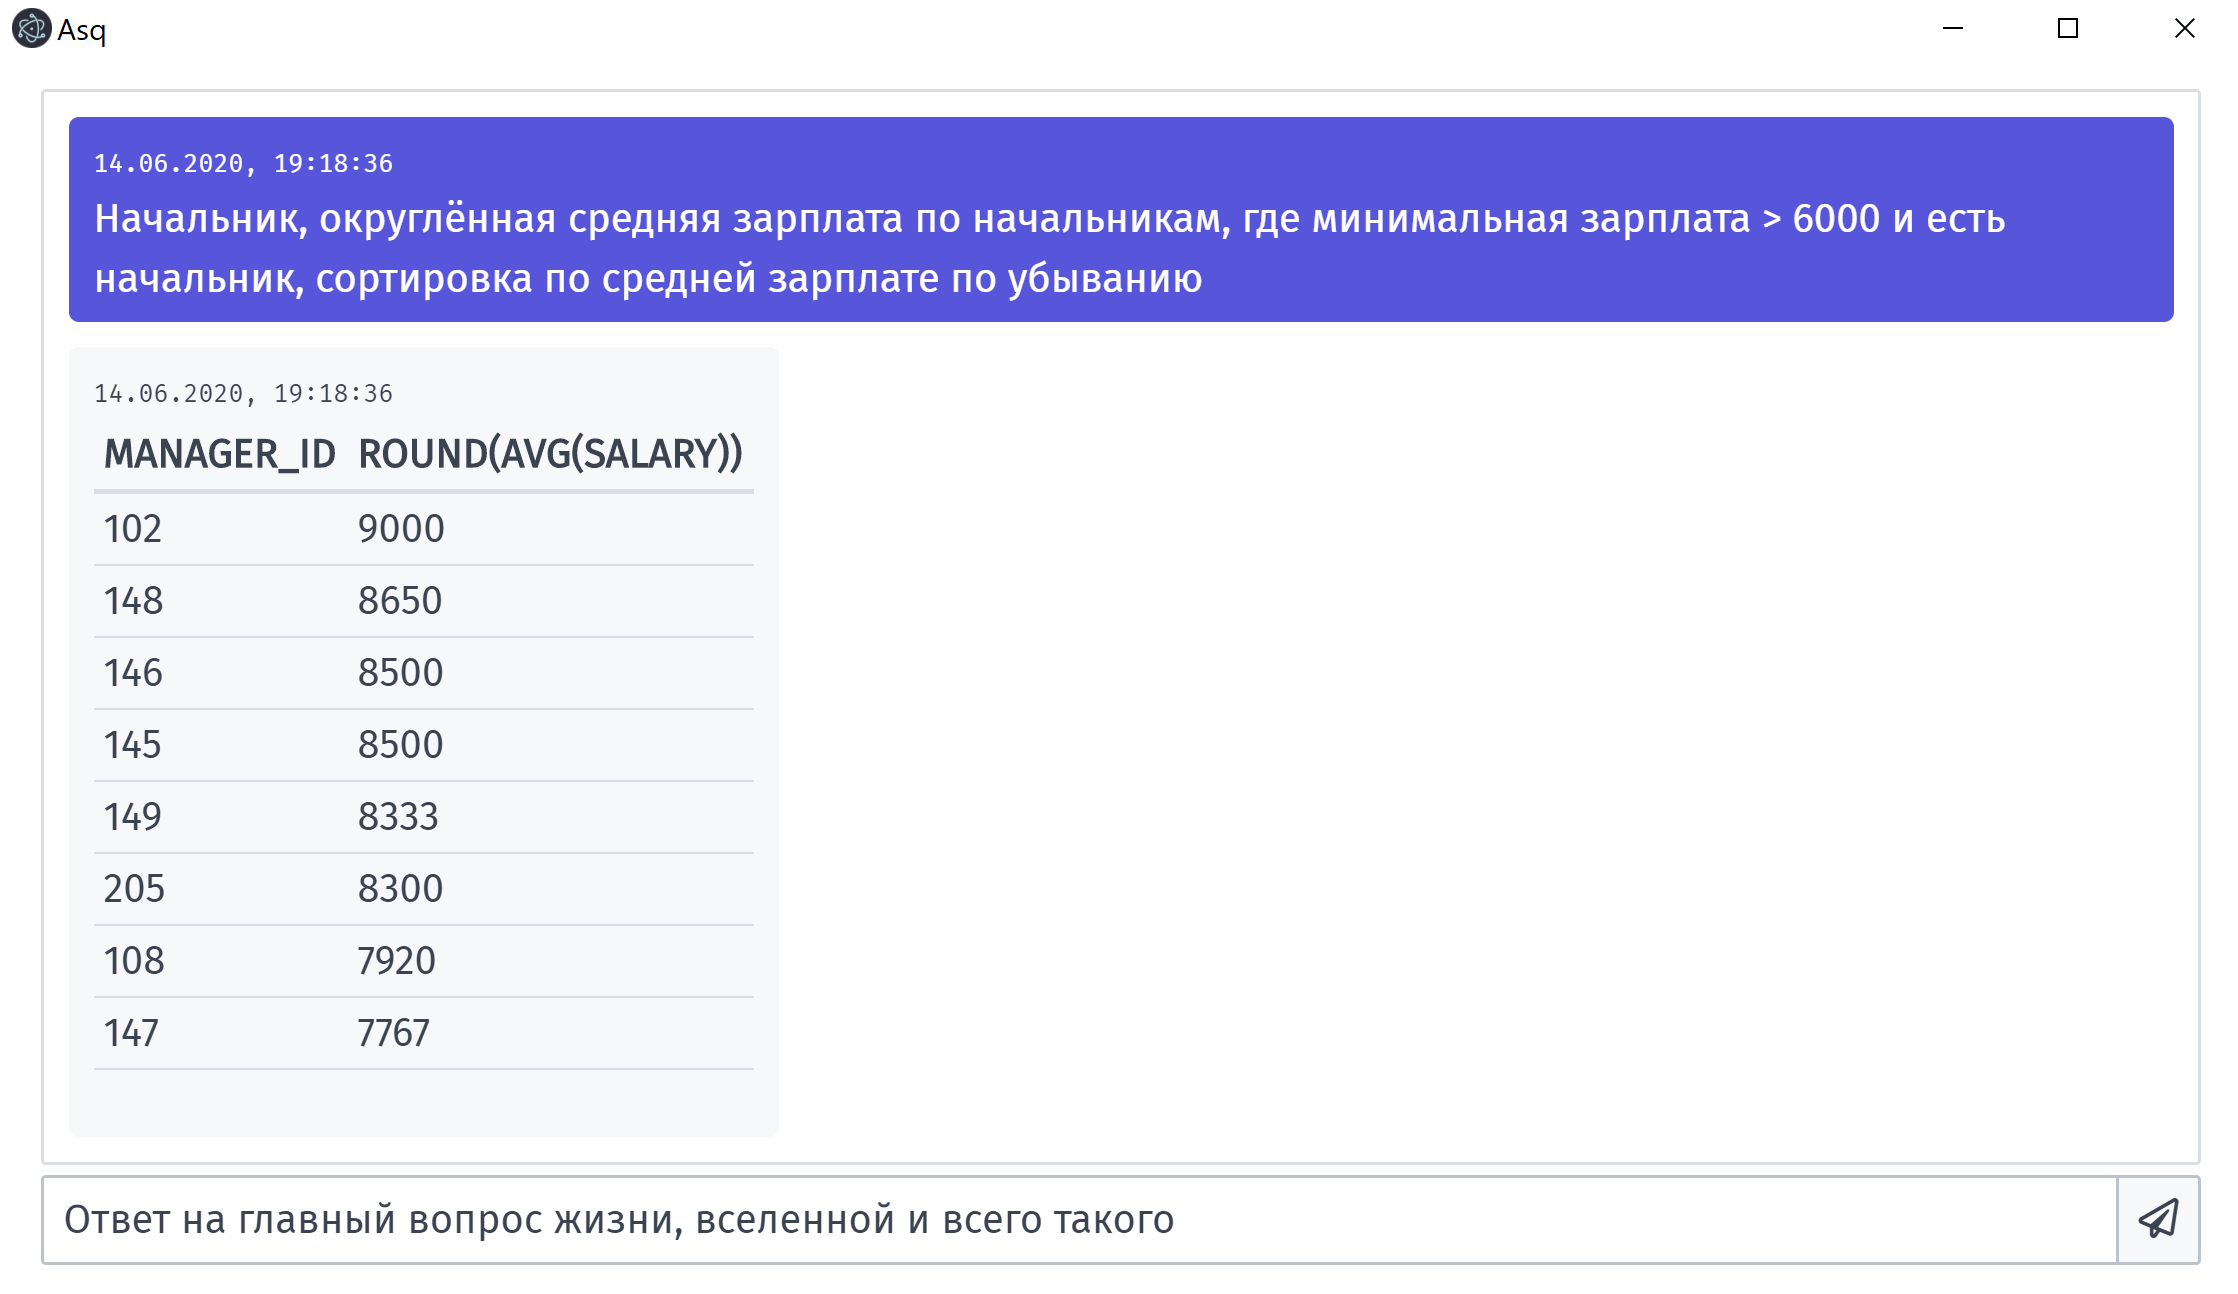
\includegraphics[width=0.75\textwidth]{img/UI.png}
  \end{center}
\end{frame}

  % %!TeX root = ../Asq.tex
\begin{frame}[fragile]{Сервер (транслятор)}%
  Транслятор поддерживает обычные и агрегатные функции, а также стандартные секции SQL:
  \texttt{SELECT}, \texttt{FROM}, \texttt{WHERE}, \texttt{GROUP BY}, \texttt{HAVING} и \texttt{ORDER BY}.
  Возможна работа как с одной, так и несколькими таблицами (\texttt{JOIN}).

  Тестирование проводилось на одной из стандартных схем Oracle "--- HR.
  \begin{center}%
    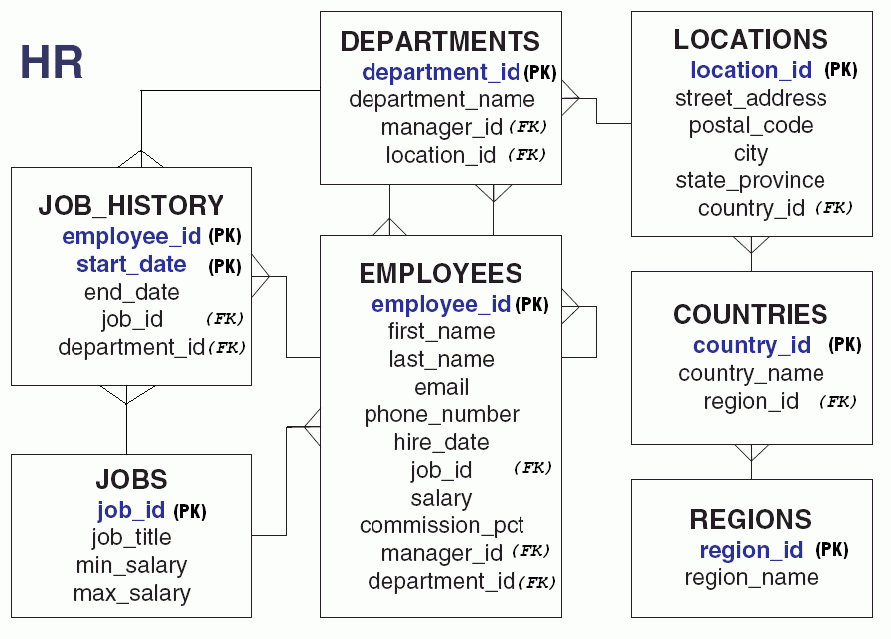
\includegraphics[width=0.4\textwidth]{img/scheme.png}
  \end{center}

\end{frame}

  % %!TeX root = ../Asq.tex
\begin{frame}[fragile]{Синонимы объектов. Пример запроса}%
  Для работы транслятора нужно задать синонимы названий столбцов и таблиц на русском языке.

  Сгенерированный код для запроса «\textit{Сколько $ \underbrace{\text{сотрудников}}_{\text{employees}} $ без $ \underbrace{\text{менеджера}}_{\text{manager\_id}} $?}»:

  \begin{minted}[tabsize=2, mathescape, fontsize=\footnotesize]{sql}
SELECT COUNT(*)
FROM hr.employees
WHERE manager_id IS NULL
  \end{minted}

\end{frame}

  % %!TeX root = ../Asq.tex
\begin{frame}[fragile]{Запрос с соединением таблиц}%
  Для всех таблиц автоматически вычисляются минимальные пути до других таблиц.

  Сгенерированный код для запроса «\textit{$ \underbrace{\text{Имя, фамилия работника}}_{\text{employees}} $ и $ \underbrace{\text{страна}}_{\text{countries}} $}»:

  \begin{minted}[tabsize=2, mathescape, fontsize=\footnotesize]{sql}
SELECT "t-1".first_name, "t-1".last_name, "t-4".*
FROM hr.employees "t-1"
  JOIN hr.departments "t-2" ON "t-1".department_id = "t-2".department_id
  JOIN hr.locations "t-3" ON "t-2".location_id = "t-3".location_id
  JOIN hr.countries "t-4" ON "t-3".country_id = "t-4".country_id
  \end{minted}

\end{frame}

  % %!TeX root = ../Asq.tex
\begin{frame}[fragile]{Различные формулировки запроса}%
  Оба запроса:
  \begin{enumerate}%
    \item «\textit{Выведи фамилию, имя и зарплату сотрудников с зарплатой больше 10000 или именем = 'David', отсортируй по зарплате по убыванию и по имени}»;
    \item «\textit{Сортировка по заработку по убыванию и имени, причём зарплата выше 10000 или имя равно 'David', вывести нужно фамилию, имя и оклад}»;
  \end{enumerate}
  "--- дают одинаковый результат:

  \begin{minted}[tabsize=2, mathescape, fontsize=\footnotesize]{sql}
SELECT last_name, first_name, salary
FROM hr.employees
WHERE salary > 10000
  -- здесь неявно для пользователя используются TRIM и LOWER.
  OR TRIM(LOWER(first_name)) = TRIM(LOWER('David'))
ORDER BY salary DESC, first_name
  \end{minted}

\end{frame}

  % %!TeX root = ../Asq.tex
\begin{frame}[fragile]{\texttt{WHERE} и \texttt{HAVING}. Группировка}%
  В SQL есть 2 вида условий: \texttt{WHERE} и \texttt{HAVING}.
  Транслятор автоматически определяет тип условия по наличию агрегатной функции.

  Сгенерированный код для запроса «\textit{Выведи начальников, округлённую среднюю зарплату по начальникам, где минимальная зарплата > 6000 и есть менеджер, отсортируй по средней зарплате по убыванию}»:

  \begin{minted}[tabsize=2, mathescape, fontsize=\footnotesize]{sql}
SELECT manager_id, ROUND(AVG(salary))
FROM hr.employees
WHERE manager_id IS NOT NULL
GROUP BY manager_id
HAVING MIN(salary) > 6000
ORDER BY AVG(salary) DESC
  \end{minted}

\end{frame}

  % %!TeX root = ../Asq.tex
\begin{frame}{Заключение}%
  \begin{itemize}%
    \item Была изучена предметная область,
    \item были исследованы методы анализа и формализации русского языка,
    \item была разработана система трансляции запросов на русском языке в SQL-код,
    \item разработанная система была протестирована на запросах различной сложности.
  \end{itemize}
\end{frame}



  % \begin{minted}[tabsize=2, mathescape, fontsize=\footnotesize]{sql}
  %   SELECT last_name, first_name, salary
  %   FROM hr.employees
  %   WHERE TRIM(LOWER(first_name)) = TRIM(LOWER('David'))
  %     OR salary > 10000
  %   ORDER BY salary DESC, first_name;
  % \end{minted}
\end{document}